\documentclass{article}

\usepackage[utf8]{inputenc}
\usepackage[T1]{fontenc}      
\usepackage[francais]{babel}
\usepackage{chemist}
\usepackage{chemfig} 
\usepackage{lewis}
\usepackage[top=2.5cm,bottom=2.5cm,right=2.5cm,left=2.5cm]{geometry}
\usepackage[squaren, Gray]{SIunits}
\usepackage{url}
\usepackage{hyperref}
\hypersetup{
    colorlinks,
    citecolor=black,
    filecolor=black,
    linkcolor=black,
    urlcolor=black
}

\newcommand\chemfigc[1]{
\vspace{0.5cm}
\begin{center}\chemfig{#1}\end{center}
\vspace{0.5cm}}

\title{Projet 3 - Rapport de tâche 1}
\author{\textbf{Groupe 124.3}
\\
\textsc{Frenyo} P\'eter (6266-12-00)\\
\textsc{Gillain} Nathan (7879-12-00)\\
\textsc{Lamine} Guillaume (7109-13-00)\\
\textsc{Piraux} Pauline (2520-13-00)\\
\textsc{Paris} Antoine (3158-13-00)\\
\textsc{Quiriny} Simon (4235-13-00)\\
\textsc{Schrurs} Sébastien (7978-13-00)}
\date{\today} 
\begin{document}

\maketitle
\tableofcontents

\section{Calcul du flux des réactifs}

\paragraph{Hypothèse}
Lors du calcul de ces flux, nous avons utilisé l'hypothèse que tous les réactifs sont 
consommés par le réacteur.

\paragraph{Calculs}
L'équation de la réaction de production de l'ammoniac par le procédé \textsc{Haber-Bosch} est donnée par :

	\begin{chemmath}
			\frac{1}{2}N_2(g) + \frac{3}{2}H_2(g) \longrightarrow NH_3(g) + \Delta H
 	\end{chemmath}
	
En sachant que l'on cherche à produire \unit{1000}{\ton} de \chemform{NH_3} par jour, 
on calcule assez facilement le flux de \chemform{N_2} (les détails de calculs ont été omis
dans ce rapport)

	$$m_{N_2} = \unit{823.5}{\ton\per\dday}$$

et le flux de \chemform{H_2}

	$$m_{H_2} = \unit{176.4}{\ton\per\dday}.$$

\section{Calcul du débit d'eau nécessaire pour refroidir le réactif}
\paragraph{Hypothèses}
\begin{itemize}
	\item Les capacités calorifiques ne dépendent pas de la température ;
	\item La pression dans le réacteur est constante et vaut \unit{10^5}{\pascal}.
\end{itemize}

\paragraph{Première méthode : on considère les capacités calorifiques constantes}
Pour la réaction donnée dans la section précédente, on a $\Delta H(\unit{298.15}{\kelvin})
 = \unit{-46 \cdot 10^3}{\joule}$ pour une mole de \chemform{NH_3(g)} produite \cite{atkins}.
Comme la réaction a lieu à \unit{500}{\celsius} (c'est à dire \unit{773.15}{\kelvin}), il
va falloir calculer $\Delta H(\unit{773.15}{\kelvin})$. Pour cela, nous avons besoin
des capacités calorifiques moyenne à pression constante de chacun des réactifs et des produits
de la réaction. Nous trouvons ces données dans une table \cite{atkins}.

	$$
	\left\{
		\begin{array}{rl}
			C_{p_{NH_3(g)}} &= \unit{37}{\joule\per\mole\kelvin}\\
			C_{p_{H_2(g)}} 	&= \unit{28.836}{\joule\per\mole\kelvin}\\
			C_{p_{N_2(g)}} 	&= \unit{29.124}{\joule\per\mole\kelvin}
		\end{array}
	\right
	$$

On a donc :

$$\Delta H(\unit{773.15}{\kelvin}) = \Delta H(\unit{298.15}{\kelvin})
+ \int_{298.15}^{773.15} C_{p_{NH_3(g)}} dT - \frac{1}{2}\int_{298.15}^{773.15} C_{p_{N_2(g)}} dT
- \frac{3}{2} \int_{298.15}^{773.15} C_{p_{H_2(g)}} dT = \unit{-5.5887 \cdot 10^4}{\joule\per\mole}$$

Pour la quantité de \chemform{NH_3} à produire par jour (à savoir $\unit{58.83 \cdot 10^6}{\mole}$),
la quantité de chaleur produite est donc :

$$q = \Delta H(\unit{773.15}{\kelvin}) \cdot n_{NH_3} = \unit{-3.28786 \cdot 10^{12}}{\joule}$$

En connaissant la capacité calorifique de l'eau $C_{H_2O(g)} = \unit{4185.5}{\joule\per\kilo\gram\kelvin}$ \cite{atkins}et en égalant
$q$ à $m_{H_2O} \cdot C_{H_2O(g)} \cdot \Delta T$ avec $\Delta T = 90 - 25 = \unit{65}{\kelvin}$, on trouve un
flux d'eau égal à

$$m_{H_2O} = \unit{1.2085 \cdot 10^7}{\kilo\gram\per\dday} \Rightarrow V_{H_2O} \approx \unit{1.2085 \cdot 10^7}{\liter\per\dday} 
= \unit{139.8}{\liter\per\second}$$

\paragraph{Deuxième méthode : les capacités calorifiques dépendent de la température}
On peut être plus précis en utilisant les capacités calorifiques suivantes \cite{hc-table} :

	$$
	\left\{
		\begin{array}{rl}
			C_{p_{NH_3(g)}}(T) &= \unit{31.81 + (15.48 \cdot 10^{-3})T + (5.86 \cdot 10^{-6})T^2}{\joule\per\mole\kelvin}\\
			C_{p_{H_2(g)}}(T) 	&= \unit{29.30 - (0.84 \cdot 10^{-3})T + (2.09 \cdot 10^{-6})T^2}{\joule\per\mole\kelvin}\\
			C_{p_{N_2(g)}}(T) 	&= \unit{27.62 + (4.19 \cdot 10^{-3})T}{\joule\per\mole\kelvin}
		\end{array}
	\right
	$$

En refaisant le calcul ci-dessus en tenant compte de la variation des capacités calorifiques en fonction
de la température, nous obtenons un débit un peu inférieur de \unit{135.662}{\liter\per\second}. On remarque
que l'approximation faite ci-dessus n'est pas si mauvaise que ça. Nous vous épargons ici
les détails de calculs (que nous avons réalisé avec \textsc{Matlab}).

\section{Sources des réactifs}
	\subsection{Sources de diazote}
	\subsubsection{Procédé cryogénique}
	Ce procédé se base sur la séparation des différents constituants de l'air en fonction de leur température 
	d'ébullition (l'oxygène \chemform{O_2} se condense avant le diazote \chemform{N_2}).
	L'air est purifié jusqu'à liquéfaction et les différents constituants sont séparés dans une colonne de 
	rectification par distillation fractionnée. Cette méthode permet d'avoir du diazote \chemform{N_2} pur 
	à \numprint{99,99}\%. Cette méthode est efficace pour une consommation au-delà de $\unit{200}{\meter\cubed\per\hour}$ \cite{scf}. 

	\subsubsection{Perméation gazeuse}
	Ce procédé utilise les différentes vitesses d'effusion des molécules de gaz à travers une membrane. 
	L'\chemform{O_2}, \chemform{H_2O} et le \chemform{CO_2} s'effusent plus rapidement que le \chemform{N_2}.
	Cette méthode nous permet d'obtenir du \chemform{N_2} sec pur à \numprint{95-99}. Ce procédé s'utilise pour des 
	débits forts variables ($\unit{3-1000}{\meter\cubed\per\hour}$) \cite{scf}.

	\subsubsection{Méthode de Ramsay}
	
	\begin{chemmath}
			NaNO_2(aq) + NH_4Cl(aq) \longrightarrow NaCl(aq) + 2 H_2O(l) + N_2(g)
	\end{chemmath}
	
	On chauffe le mélange de \chemform{NaNO_2} et \chemform{NH_4Cl} pour obtenir le \chemform{N_2} sous forme gazeuse.
	Un désavantage de cette méthode par rapport aux 2 premières est qu'il faut acheter les réactifs. De plus, il faut utiliser de l'énergie pour chauffer la réaction \cite{wiki-n2}.

	\subsection{Sources de dihydrogène}
		\subsubsection{Vaporeformage de méthane}
		2 réactions sont utilisées pour ce procédé \cite{afhypac} :
		
		\begin{chemmath} 
			CH_4 + H_2O \longleftrightarrow CO + 3H_2
		\end{chemmath}
		
		\begin{chemmath}
			CO + H_2O \longleftrightarrow CO_2 + H_2
		\end{chemmath}
		
		L'équation bilan obtenue est la suivante :
		
		\begin{chemmath}
			CH_4 + 2H_2O \longleftrightarrow CO_2 + 4 H_2
		\end{chemmath}
		
			Cette réaction nécessite un catalyseur : le nickel. Le rendement varie entre $40-45\%$. Le problème de cette 
			méthode est qu'elle rejette une grande quantité de \chemform{CO_2}, gaz à effet de serre \cite{wiki-h2}.
			
		\subsubsection{Oxydation partielle d'hydrocarbure}
		\begin{chemmath}
			C_nH_m + \frac{n}{2} O_2 + \frac{3,76n}{2} N_2 \longrightarrow \frac{m}{2} H_2 + n CO + \frac{3,76n}{2} N_2
		\end{chemmath}
		L'air est comburant pour cette réaction, qui a besoin d'être catalysée. Son caractère exothermique aide à la catalyse. 
		L'inconvénient de cette méthode est son faible rendement \cite{wiki-h2}.

		\subsubsection{Electrolyse}
		Réaction à l'anode : 
		
		\begin{chemmath}
			2H_2O(l) \longrightarrow O_2(g) + 4 H^+(aq) + 4e^-
		\end{chemmath}
		
		Réaction à la cathode :
		
		\begin{chemmath}
			4H_2O(l) + 4e^- \longrightarrow 2H_2O(g) + 4OH^-(aq)
		\end{chemmath}
		
		L'équation bilan obtenue est la suivante :
		
		\begin{chemmath}
			2H_2O(l) \longrightarrow 2H_2(g) + O_2(g)
		\end{chemmath}
		
	La réaction nécessite une grande quantité d'électricité. L'eau, quant à elle, est présente en quantité illimitée 
	et est peu coûteuse. En pratique, cette méthode est très peu utilisée \cite{wiki-h2}.
	
	\section{Premier jet du flow-sheet simplifié}
	La première ébauche de notre flow-sheet se trouve à la figure \ref{flow-sheet}.
	
	\begin{figure}[htb!]
		\centering
		\rotatebox{90}{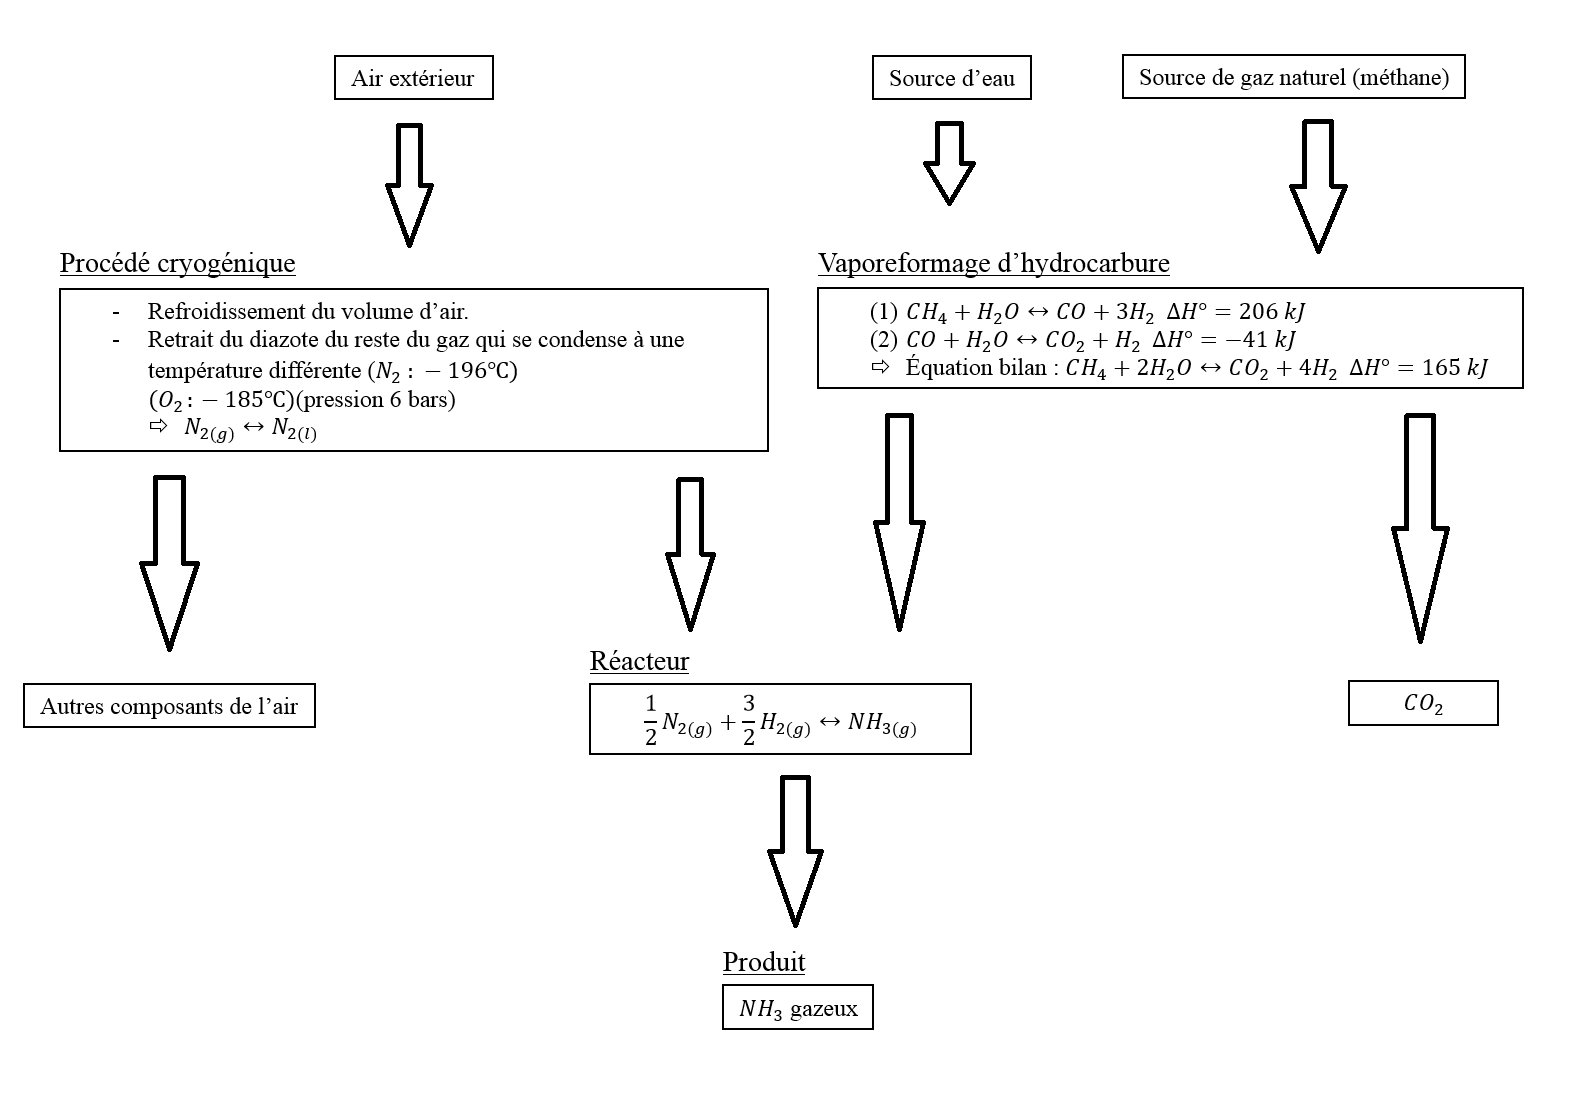
\includegraphics[scale=0.50]{flow-sheet.png}}
		\caption{Première ébauche de notre flow-sheet.}
		\label{flow-sheet}
	\end{figure}
	
	\section{Deuxième version du flow-sheet}
	Voici la deuxième version du flow-sheet (Figure \ref{flow-sheet-v2}).
	
	\begin{figure}[htb!]
	\centering
	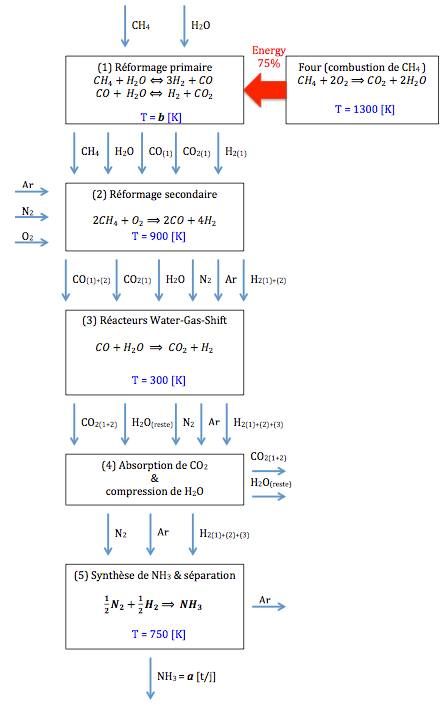
\includegraphics[scale=0.80]{flow-sheet-v2.jpg}
	\caption{Deuxième ébauche de notre flow-sheet.}
	\label{flow-sheet-v2}
	\end{figure}

\section{Bilan de matiere}
On pose le flux de \chemform{NH_3(g)} à la sortie égal à $\unit{m_{NH_3}}{\gram\per\dday}$. 

Nous partons de la réaction : 
\begin{chemmath}
		\frac{1}{2}N_2(g) + \frac{3}{2}H_2(g) \longrightarrow NH_3(g) 
\end{chemmath}
 	
$$m_{NH_3} = \unit{m_{NH_3}}{\gram\per\dday}$$ 

Et donc, 
 
$$n_{NH_3} = \unit{\frac{m_{NH_3}}{17}}{\mole}$$

Ce qui donne 

$$n_{N_2} = \frac{n_{NH_3}}{2} = \unit{\frac{m_{NH_3}}{34}}{\mole}$$ 

et 

$$n_{H_2} = \frac{3}{2} \cdot n_{NH_3}$$

On sait que le \chemform{N_2(g)} provient uniquement de l'air entrant 
dans le réacteur du  réformage primaire. Et comme on peut considérer
que l'air est composé de 78\% de \chemform{N_2(g)}, 21\% de \chemform{O_2(g)}
et 1\% d'\chemform{Ar(g)}, on peut déduire que $$n_{air}$$ entrant dans le 
réacteur du réformage primaire vaut : 

$$n_{air}= n_{N_2} \cdot \frac{100}{78} = \unit{\frac{25m_{NH_3}}{663}}{\mole}$$ 

Et :
$$n_{O_2}= n_{air} \cdot \frac{21}{100} = \unit{\frac{7m_{NH_3}}{884}}{\mole}$$
$$n_{Ar}= n_{air} \cdot \frac{1}{100} = \unit{\frac{1m_{NH_3}}{2652}}{\mole}$$

On sait par la réaction du réformage primaire suivante et par l'hypothèse que le
\chemform{CH_4(g)} et le \chemform{O_2(g)} sont présents en quantité stoechiométrique : 

\begin{chemmath}
	2CH_4 + O_2 \Longrightarrow 2CO + 4 H_2
\end{chemmath} 

que :

$$n_{CH_4} = 2 \cdot n_{O_2} = \unit{\frac{7m_{NH_3}}{442}}{\mole}$$
$$n_{CO} = n_{CH_4} =  \unit{\frac{7m_{NH_3}}{442}} {\mole}$$
$$n_{H_2} = 2 \cdot n_{CH_4} =  \unit{\frac{7m_{NH_3}}{221}}{\mole}$$

On s'intéresse ensuite à la réaction du Water-Gas-Shift : 

\begin{chemmath}
	CO + H_2O \Longrightarrow CO_2 + H_2
\end{chemmath} 

On sait que $n_{CO}$ du WGS = $n_{CO}$ produit au réformage primaire
$+ n_{CO}$ produit au réfomarge secondaire. 

Et donc on a : 

$$n_{CO_2} = n_{CO} = n_{H_2O}$$

S'il reste du \chemform{H_2O} à la fin de cette réaction, $n_{H2_O}$ 
sera égal à $n_{H2_O}$ du réformage primaire moins le $n_{CO}$ du WGS.

On peut aussi déduire que $n_{CO_2-tot} = n_{{CO_2}-\text{réformage primaire}}
+ n_{{CO_2}-\text{WGS}}$.

On peut aussi conclure que : 

$$n_{H_2-\text{réformage primaire}}= n_{H_2-\text{synthèse} \chemform{NH_3}}
- n_{H_2-\text{réformarge secondaire}} - n_{H_2-\text{WGS}}$$

% A transformer en tableau pour plus que ce soit plus clair.
Après la résolution de l'équilibre du réformage primaire, 
on obtient les valeurs suivantes : 

$$n_{H_2O-\text{réformage primaire}} = $$
$$n_{CO-\text{réformage primaire}} = $$
$$n_{CO_2-\text{réformage primaire}} = $$
$$n_{H_2-\text{réformage primaire}} = $$

$$n_{CO-\text{WGS}} = $$
$$n_{CO2-\text{WGS}} = $$
$$n_{H_2-\text{WGS}} = $$

$$n_{CO_2-\text{final}} = $$ 
$$n_{H_2O-\text{final}} = $$

\section{Equilibre du reformage primaire}
\subsection{Calcul de la constante d'équilibre}

Pour calculer la constante d'équilibre nous allons utiliser $K= \exp{\frac{-\Delta G}{RT}}$ avec $\Delta G = \Delta H - T \Delta S $

\subsubsection{Première équation}
\begin{chemmath} 
 CH_4(g) + H_{2}O(g) \longrightarrow CO(g) + 3H_2
\end{chemmath} 

Connaissant les capacités calorifiques dépendantes de la température:
$$
\left\{
	\begin{array}{rl}
		C_{p_{CO}}(T) 			&= \unit{27.62 +(5.02 \cdot 10^{-3})T}{\joule\per\mole\kelvin} \\
		C_{p_{H_{2}}}(T) 		&= \unit{29.3-(0.84 \cdot 10^{-3})T + (2.09\cdot 10^{-6})T^2}{\joule\per\mole\kelvin} \\
		C_{p_{CH_{4}}}(T) 	&= \unit{14.23+(75.3 \cdot 10^{-3})T - (18\cdot 10^{-6})T^2}{\joule\per\mole\kelvin} \\
		C_{p_{H_{2}O}}(T) 	&= \unit{30.13+(10.46 \cdot 10^{-3})T}{\joule\per\mole\kelvin} 
	\end{array}
\right
$$

$$
\Delta H_1(T) = \Delta H(\unit{298.15}{\kelvin}) 
 + \int_{298.15}^{T} C_{p_{CO(g)}} dT + 3\int_{298.15}^{T} C_{p_{H_2(g)}} dT 
 +  \int_{T}^{298.15} C_{p_{CH_4(g)}} dT + \int_{T}^{298.15}C_{p_{H_{2}O_{(g)}}}dT
 $$\\
  
 $$
 = 188369.87 + 71.16 T -0.04163 T^2 + (8.09\cdot 10^{-6}) T^3
 $$ 
 
 $$
 \Delta S_1(T) = \Delta S(\unit{298.15}{\kelvin}) 
 + \int_{298.15}^{T} C_{p_{CO(g)}} \dfrac{dT}{T} + 3\int_{298.15}^{T} C_{p_{H_2(g)}} \dfrac{dT}{T} 
 +  \int_{T}^{298.15} C_{p_{CH_4(g)}} \dfrac{dT}{T} + \int_{T}^{298.15}C_{p_{H_{2}O_{(g)}}}\dfrac{dT}{T}
 $$\\ 
 
 $$
 = -167.05 + 71.16 \ln T -0.08326 T + (1.2135\cdot 10^{-5} T^2
 $$ 
 
 $$
 \Delta G_1(T) = 188369.9 - (71.16\ln T)T + 238.21T + 0.04163 T^2 -(4.045\cdot 10^{-6}T^3
 $$ 

Nous obtenons donc
$$K_1 = \exp{\frac{-\Delta G_1}{RT}}$$
avec la valeur de $\Delta G_1$ calculée plus tôt.

\subsubsection{Deuxième équation}
\begin{chemmath} 
 CO(g) + H_{2}O(g) \longrightarrow CO_2(g) + H_2
\end{chemmath} 

Connaissant les capacités calorifiques dépendantes de la température de l'équation précedente et celle-ci:

$$
\begin{array}{rl}
C_{p_{CO_2}}(T)=32.22 +(22.18 \cdot 10^{-3})T + (3.35 \cdot 10^{-6})T^2\\
\end{array}
$$

$$
\Delta H_2(T) = \Delta H(\unit{298.15}{\kelvin}) 
 + \int_{298.15}^{T} C_{p_{CO_2(g)}} dT + \int_{298.15}^{T} C_{p_{H_2(g)}} dT 
 +  \int_{T}^{298.15} C_{p_{CO(g)}} dT + \int_{T}^{298.15}C_{p_{H_{2}O_{(g)}}}dT
 $$\\
  
 $$
 = -42533.33+3.77T+(2.93\cdot 10^-3)T^2-(4.2\cdot 10^-7)T^3
 $$ 

$$
\Delta S_2(T) = \Delta S(\unit{298.15}{\kelvin}) 
 + \int_{298.15}^{T} C_{p_{CO_2(g)}} \dfrac{dT}{T} + 3\int_{298.15}^{T} C_{p_{H_2(g)}} \dfrac{dT}{T} 
 +  \int_{T}^{298.15} C_{p_{CO(g)}} \dfrac{dT}{T} + \int_{T}^{298.15}C_{p_{H_{2}O_{(g)}}}\dfrac{dT}{T}
 $$\\
  
 $$
 = -65.9 + 3.77 \ln(T) +(5.86\cdot 10^{-3})T -(6.3 \cdot 10^{-7})T^2
 $$ 
 
 $$
 \Delta G_2=-42533.33 - (3.77 \ln(T))T +69.67 T -(2.93 \cdot 10^{-3})T^2
 + (2.1\cdot 10^{-7})T^3 
 $$
 
Nous obtenons donc
$$K_2 = \exp{\frac{-\Delta G_2}{RT}}$$
avec la valeur de $\Delta G_2$ calculée plus tôt.

\section{Bilan d'energie}
% La partie que Sébastien a envoyé par mail. A relire et vérifier.
% A remettre en bonne forme également.
\paragraph{Equation de combustion}
\begin{chemmath}
	CH_4 + 2O_2 \Longrightarrow CO_2 + 4 H_2O
\end{chemmath}

$\Delta H_{reaction} 	= \Sigma \Delta H_{f,produits} - \Sigma \Delta H_{f,reactifs}\\
						= ((-393.51) + (2\cdot(-241.82))) - ((-74.81) + 2\cdot 0))\\
						= (-877.15) - (-74.81)\\
						= \unit{-802.34}{\kilo\joule\per\mole}$

\paragraph{Reformage primaire}
\begin{chemmath}
 CH_4 + 2H_2O \Longleftrightarrow 4H_2 + CO_2
\end{chemmath}

$\Delta H_{reaction} 	= \Sigma \Delta H_{f,produits} - \Sigma \Delta H_{f,reactifs}\\
						= (4\cdot0 + (-393.51)) - (-74.81 + 2\cdot(-241.82))\\
						= (-393.51) - (-558.45)\\
						= \unit{164.94}{\kilo\joule\per\mole} $		

\paragraph{Reformage secondaire}
\begin{chemmath}
	CH_4 + \frac{1}{2}O_2 \Longrightarrow CO + 2H_2
\end{chemmath}

$\Delta H_{reaction} 	= \Sigma \Delta H_{f,produits} - \Sigma \Delta H_{f,reactifs}\\
						= ((-110.53)) + (2\cdot 0)) - ((-74.81) + \frac{1}{2}\cdot 0))\\
						= (-110.53) - (-74.81)\\
						= -\unit{35.72}{\kilo\joule\per\mole}$

Le reformage secondaire s'opere generalement a une temperature de $\unit{1173}{\kelvin}$.
Calculons les $C_p$ des differents composants a cette temperature :
$\\C_{p_{CH_{4}}}(\unit{1173.15}{\kelvin}) :\\ 14.23 + 75.3\cdot10^{-3}T + (-18\cdot10^{-6})T^2
 = 14.23 + 75.3\cdot10^{-3}\cdot1173.15 + (-18\cdot10^{-6})\cdot(1173.15)^2
 = 14.23 + 88.34 - 24.77
 = \unit{77.8}{\joule\per\mole\per\kelvin}$
 
$\\C_{p_{O_{2}}}(\unit{1173.15}{\kelvin}) :\\ 25.73 + 12.97\cdot10^{-3}T + (-3.77\cdot10^{-6})T^2
 = 25.73 + 12.97\cdot10^{-3}\cdot1173.15 + (-3.77\cdot10^{-6})\cdot(1173.15)^2
 = 25.73 + 15.22 - 5.19
 = \unit{35.76}{\joule\per\mole\per\kelvin}$
 
$\\C_{p_{CO}}(\unit{1173.15}{\kelvin}) :\\ 27.62 + 5.02\cdot10^{-3}T + (0\cdot10^{-6})T^2
 = 27.62 + 5.02\cdot10^{-3}\cdot1173.15
 = 27.62 + 5.89
 = \unit{33.5}{\joule\per\mole\per\kelvin}$
 
$\\C_{p_{H_{2}}}(\unit{1173.15}{\kelvin}) :\\ 29.3 + (-0.84)\cdot10^{-3}T + (2.09\cdot10^{-6})T^2
 = 29.3 - 0.84\cdot10^{-3}\cdot1173.15 + (2.09\cdot10^{-6})\cdot(1173.15)^2
 = 29.3 - 0.98 + 2.88
 \\= \unit{31.19}{\joule\per\mole\per\kelvin}$

Calculons maintenant le $\Delta H$ a $\unit{1173.15}{\kelvin}$ :

$$\Delta H(\unit{1173.15}{\kelvin}) = \Delta H(\unit{298.15}{\kelvin}) 
+ \int_{1173.15}^{298.15} C_{p_{reactifs}} dT + \int_{298.15}^{1173.15} C_{p_{produits}} dT$$

$ \\= \Delta H(\unit{298.15}{\kelvin}) + \int_{1173.15}^{298.15} C_{p_{CH_{4}}} dT +\frac{1}{2}\int_{1173.15}^{298.15} C_{p_{O_{2}}} dT + \int_{298.15}^{1173.15} C_{p_{CO}} dT + 2\int_{1173.15}^{298.15} C_{p_{H_{2}}} dT$
$ \\= -35.72 kJ/mol 
+\int_{1173.15}^{298.15} (14.23 + 75.3*10^{-3}T + (-18*10^{-6})T^2) dT 
+\frac{1}{2}\int_{1173.15}^{298.15} (25.73 + 12.97*10^{-3}T + (-3.77*10^{-6})T^2) dT
+\int_{298.15}^{1173.15} (27.62 + 5.02*10^{-3}T + (0*10^{-6})T^2) dT 
+2\int_{298.15}^{1173.15} (29.3 + (-0.84)*10^{-3}T + (2.09*10^{-6})T^2) dT$			
$ \\= -35.72 kJ/mol 
- [14.23T + \frac{75.3*10^{-3}}{2}T^2 + (\frac{-18*10^{-6}}{3})T^3]_{298.15}^{1173.15} 
-\frac{1}{2} [25.73T + \frac{12.97*10^{-3}}{2}T^2 + (\frac{-3.77*10^{-6}}{3})T^3]_{298.15}^{1173.15} 
+ [27.62T + \frac{5.02*10^{-3}}{2}T^2 + \frac{(0*10^{-6})}{3}T^3]_{298.15}^{1173.15}  
+2 [29.3T + \frac{(-0.84)*10^{-3}}{2}T^2 + \frac{(2.09*10^{-6})}{3}T^3]_{298.15}^{1173.15} $
$ \\= -35720
-(58823.4-7430.5) -\frac{1}{2}(37081-8214.57)+(35856.9-8458.03)+2(34920.1-7986.16)$		
$ \\= -35720 - 51392.9 - 14433.215 + 27398.87 + 53867.88 $
$ \\= -20279.365 J $
		
Water-Gas-Shift :
\begin{chemmath}
	CO + H_2O \Longrightarrow H_2 + CO_2
\end{chemmath}	

$\Delta H_{reaction} 	= \Sigma \Delta H_{f,produits} - \Sigma \Delta H_{f,reactifs}\\
						= (0 + (-393.51)) - (-110.53 + (-241.82))\\
						= (-393.51) - (-352.35)\\
						= -41.16 kJ/mol $

Le Water Gas Shift s'opere generalement entre 200 et \unit{400}{\degree}. Nous considererons alors une temperature de reaction de $\unit{300}{\degree}$, soit $\unit{573.15}{\kelvin}$.
						
Calculons les $C_{p}$ des differents composants a cette temperature :
						
$\\C_{p_{CO}}(\unit{573.15}{\kelvin}) :\\ 27.62 + 5.04*10^{-3}*T + (0*10^{-6})*T^2
 = 27.62 + 5.04*10^{-3}*573.15 + (0*10^{-6})*(1173.15)^2
 = 27.62 + 2.89
 \\= 30.5 (J.mol^{-1}.K^{-1})$	
 
$\\C_{p_{H_{2}O}}(\unit{573.15}{\kelvin}) :\\ 30.13 + 10.46*10^{-3}*T + (0*10^{-6})*T^2
 = 30.13 + 10.46*10^{-3}*573.15 + (0*10^{-6})*(573.15)^2
 = 30.13 + 5.99
 \\= 36.12 (J.mol^{-1}.K^{-1})$ 
 

$\\C_{p_{CO_{2}}}(\unit{573.15}{\kelvin}) :\\ 32.22 + 22.18*10^{-3}*T + (-3.35*10^{-6})*T^2
 = 32.22 + 22.18*10^{-3}*573.15 + (-3.35*10^{-6})*(573.15)^2
 = 32.22 + 12.71 - 1.1
 \\= 43.83 (J.mol^{-1}.K^{-1})$ 
 					
					
$\\C_{p_{H_{2}}}(\unit{573.15}{\kelvin}) :\\ 29.3 + (-0.84)*10^{-3}*T + (2.09*10^{-6})*T^2
 = 29.3 - 0.84*10^{-3}*573.15 + (2.09*10^{-6})*(573.15)^2
 = 29.3 - 0.48 + 0.69
 \\= 29.5 (J.mol^{-1}.K^{-1})$					
					
$\\$Calculons maintenant le \Delta H a $\unit{573.15}{\kelvin}$ :				
$$\Delta H(\unit{573.15}{\kelvin}) = \Delta H(\unit{298.15}{\kelvin}) 
+ \int_{573.15}^{298.15} C_{p_{reactifs}} dT + \int_{298.15}^{573.15} C_{p_{produits}} dT$$


$ \\= \Delta H(\unit{298.15}{\kelvin}) + \int_{573.15}^{298.15} C_{p_{CO}} dT +\int_{573.15}^{298.15} C_{p_{H_{2}O}} dT + \int_{298.15}^{573.15} C_{p_{CO_{2}}} dT + \int_{298.15}^{573.15} C_{p_{H_{2}}} dT$
$ \\= -41.16 kJ/mol 
+\int_{573.15}^{298.15} (27.62 + 5.04*10^{-3}T + (0*10^{-6})T^2) dT 
+\int_{573.15}^{298.15} (30.13 + 10.46*10^{-3}T + (0*10^{-6})T^2) dT
+\int_{298.15}^{573.15} (32.22 + 22.18*10^{-3}T + (-3.35*10^{-6})T^2) dT 
+\int_{298.15}^{573.15} (29.3 + (-0.84)*10^{-3}T + (2.09*10^{-6})T^2) dT$			
$ \\= -41.16 kJ/mol 
- [27.62T + \frac{5.04*10^{-3}}{2}T^2 + (\frac{0*10^{-6}}{3})T^3]_{298.15}^{573.15} 
- [30.13T + \frac{10.46*10^{-3}}{2}T^2 + (\frac{0*10^{-6}}{3})T^3]_{298.15}^{573.15} 
+ [32.22T + \frac{22.18*10^{-3}}{2}T^2 + \frac{(-3.35*10^{-6})}{3}T^3]_{298.15}^{573.15}  
+ [29.3T + \frac{(-0.84)*10^{-3}}{2}T^2 + \frac{(2.09*10^{-6})}{3}T^3]_{298.15}^{573.15} $
$ \\= -41160
-(16658.2-8458.91)-(18987.1-9448.17)+(21899.7-10562.6)+(16786.5-8716.92)$		
$ \\= -41160 - 8199.29 - 9538.93 + 11337.1 + 8069.58 $
$ \\= -55630.7 J $

\section{Outil de gestion}
% To do

\section{Calcul du nombre de tuyaux}
Maintenant, nous allons calculer le nombre de tubes dont nous aurons
besoin pour notre réacteur multi-tubulaire. Nous avons ces données de base :
$\dot{m_{NH_{3}}} = \unit{1500}{\ton\per\dday}$, $d_{tube} = \unit{10^{-1}}{\meter}$ 
et $c = \unit{2}{\meter\per\second}$ où $\dot{m_{NH_{3}}}$ est le débit massique par
jour d'ammoniac, $d_{tube}$ est le diamètre d'un tube et $c$ est la vitesse superficielle
à l'entrée du réacteur. Transformons d'abord le débit massique en débit volumique.

$$ \unit{1500}{\ton\per\dday} =  \unit{1.736\cdot 10^{-2}}{\ton\per\second} = 
\unit{17.36 \cdot v}{\meter^{3}\per\second} = \dot{V} $$

avec $v$ le volume massique (en \unit{}{\meter\cubed\per\kilo\gram}) du mélange que l'on introduit dans le réacteur. 
Nous pouvons déterminer $v$ grâce à l'expression de la loi des gaz parfaits 
sous forme thremodynamique $v = \frac{R^*T}{31 \cdot 10^{5}}$ où $R^*$
vaut $\frac{R}{\frac{16\cdot x_{CH_{4}}+18\cdot x_{H_{2}O}}{2}}}$ ($x_{CH_{4}$ 
et $x_{H_{2}O}$ sont les fractions molaire du méthane et de l'eau entrant dans le système).
Ensuite, à l'aide des notions de système ouvert et de l'hypothèse $\dot{m_{entrée}} = \dot{m_{sortie}}$, 
nous obtenons que $\dot{V} = c \cdot A$ avec $\dot{V}$ le débit volumique et $A$ 
la somme des sections de tous les tubes. En remplaçant par les valeurs que nous possédons, nous obtenons :

$$A = \frac{\dot{V}}{c} = \frac{1.736\cdot 10\cdot v}{2} = \unit{8.68\cdot v}{\meter^{2}}$$

Or, on sait que la surface d'un tube vaut $\pi\cdot(\frac{d}{2})^{2} = \unit{7.85 \cdot 10^{-3}}{\meter\squared}$. 
Le nombre de tubes est, dès lors, le rapport de la section totale trouvée plus haut sur 
la section d'un tube. Ce qui nous donne finalement : 

$$\text{Nombre de tubes} = \frac{8.68\cdot v}{7.854\cdot 10^{-3}} = 1105.17\cdot v$$

\bibliography{source-tache1}
\bibliographystyle{plain}
\nocite{*}
	
\end{document}
